\documentclass[landscape]{slides}

\usepackage[dvips]{color,epsfig}
\newcommand{\code}[1]{\texttt{#1}}
\pagestyle{empty}
\title{NachOS File System Design}
\author{Trevor Clarke\\
	Eric Eells\\
	Eric Ferguson\\
	Daniel Westgate}

\begin{document}
    \begin{slide}
	\maketitle
    \end{slide}

    \begin{slide}
	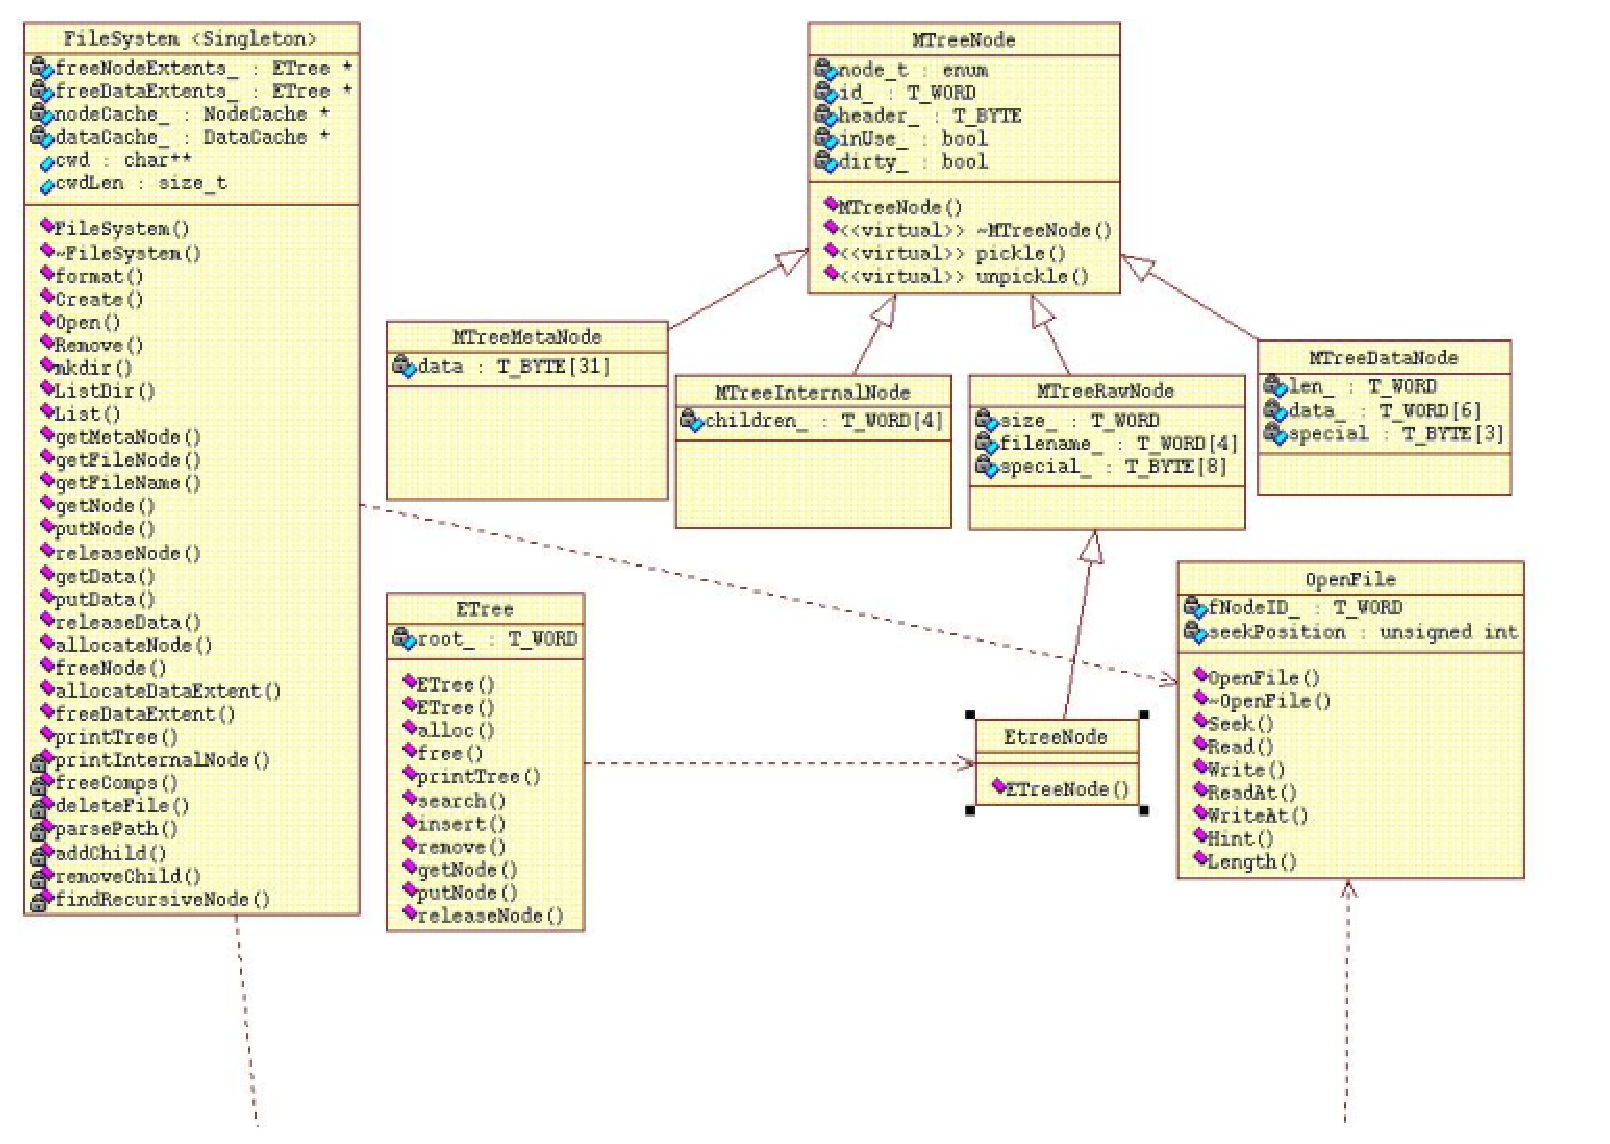
\epsfig{file=filesysTOP.eps}
    \end{slide}
    \begin{slide}
	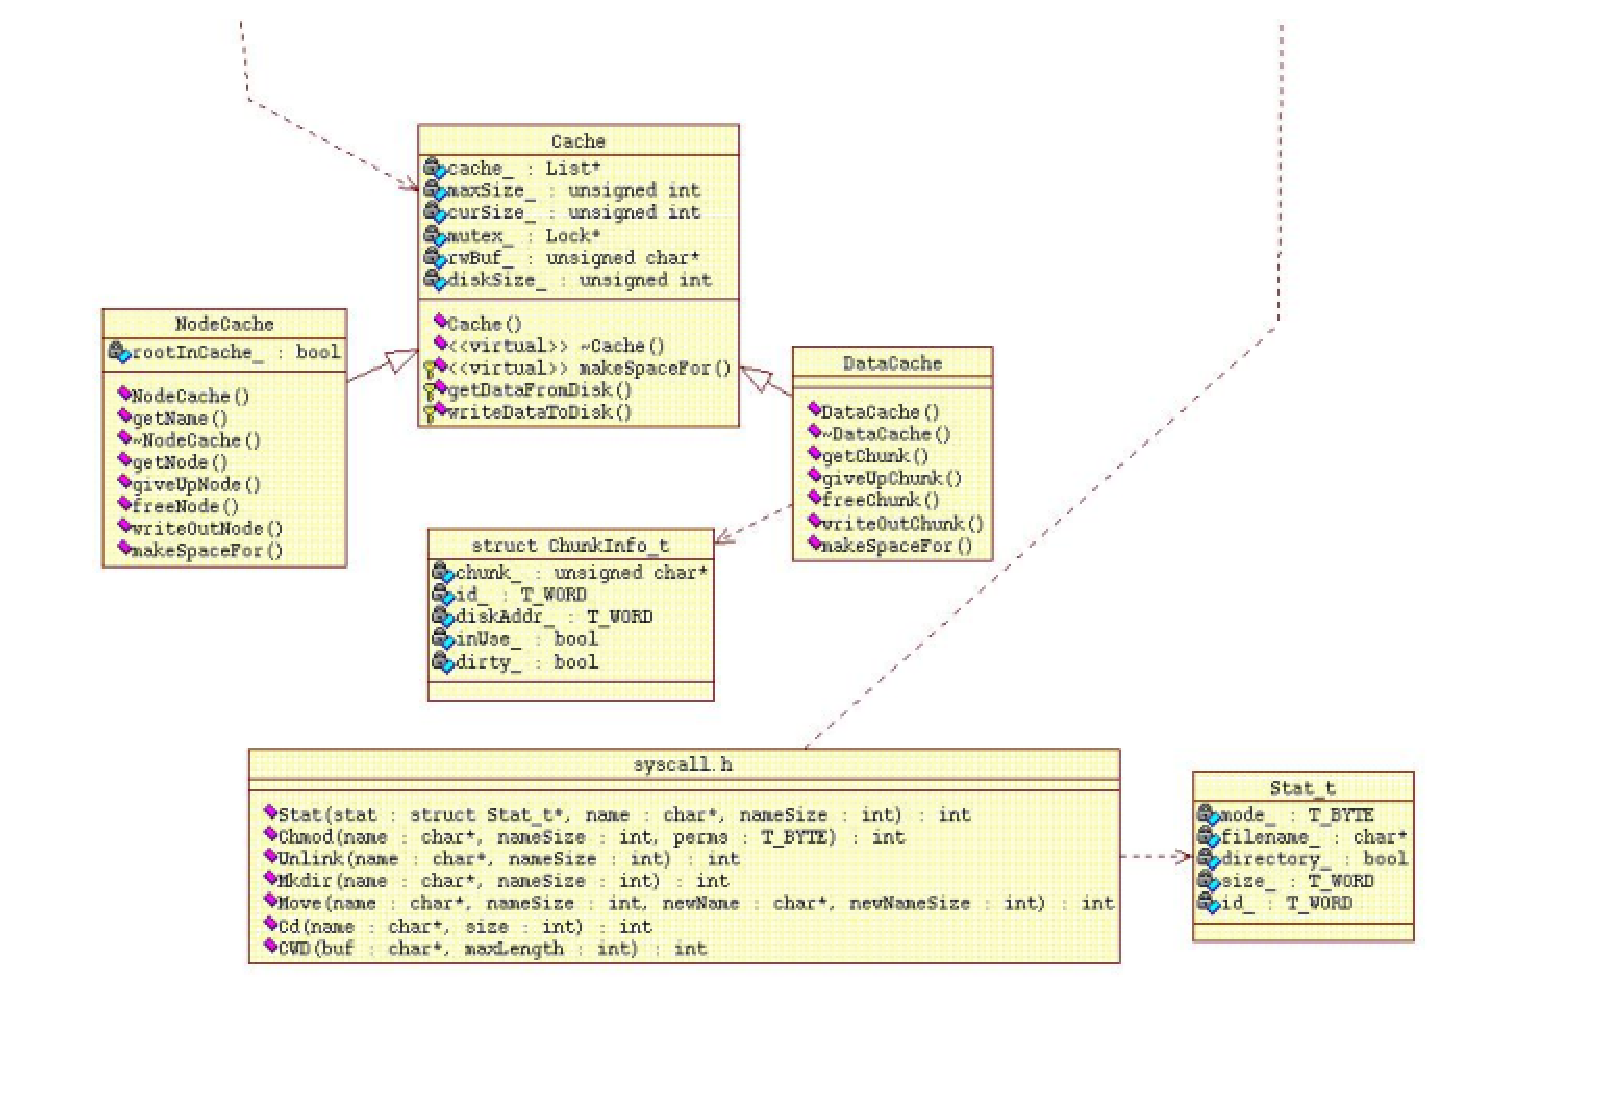
\epsfig{file=filesysBOTTOM.eps}
    \end{slide}

    \begin{slide}
	\begin{center}\large NachOS File System\end{center}
	\begin{itemize}
	    \item File System Structure
	    \item New System Calls
	    \item \code{FileSystem} \& \code{OpenFile}
	    \item \code{MTreeNode} \& \code{ETree}
	    \item \code{Cache}
	    \item Limitations
	\end{itemize}
    \end{slide}

    \begin{slide}
	\begin{center}\large File System Structure\end{center}
	\begin{itemize}
	    \item Nodes \& Data Chunks
	    \item On Disk Structure
	    \item Root Node Structure
	    \item Free Extent Trees
	\end{itemize}
    \end{slide}
    \begin{slide}
	\begin{center}\large File System Structure\end{center}
	\begin{itemize}
	    \item File Sub-tree
	    \item Directory Sub-tree
	    \item Meta Node
	    \item Data Extents \& Fragmentation
	\end{itemize}
    \end{slide}

    \begin{slide}
	\begin{center}\large New System Calls\end{center}
	\begin{itemize}\small
	  \item \code{int Stat( struct Stat\_t* stat, char* name, int nameSize )}
	  \item \code{int Chmod( char* name, int nameSize, T\_BYTE perms )}
	  \item \code{int Unlink( char* name, int nameSize )}
	  \item \code{int Mkdir( char* name, int nameSize )}
	  \item \code{int Move(char* name, int nameSize, char* newName, int newNameSize)}
	  \item \code{int Cd( char* name, int size)}
	\end{itemize}
    \end{slide}

    \begin{slide}
	\begin{center}\large \code{FileSystem} \& \code{OpenFile}\end{center}
	\begin{itemize}
	  \item \code{void format()}
	  \item \code{Create()}, \code{Read()}, \code{Write()}
	  \item \code{getFileNode()}, \code{getMetaNode()}, \code{getNode}
	  \item \code{releaseNode()}, \code{putNode()}
	  \item Data Chunks
	  \item Allocation \& Deallocation
	\end{itemize}
    \end{slide}

    \begin{slide}
	\begin{center}\large \code{MTreeNode} \& \code{ETree}\end{center}
	\begin{itemize}
	    \item Raw Node
	    \item Internal Node
	    \item Meta Node
	    \item Data Node
	    \item Extent Node
	\end{itemize}
    \end{slide}

    \begin{slide}
	\begin{center}\large \code{Cache}\end{center}
	\begin{itemize}
	    \item Requesting An Entry
	    \item Releasing An Entry
	    \item Writing An Entry
	    \item Synchronization
	\end{itemize}
    \end{slide}

    \begin{slide}
	\begin{center}\large Limitations\end{center}
	\begin{itemize}
	    \item Filename Length
	    \item Directory Children
	    \item Node/Data Distribution
	    \item Error Handling
	    \item Journaling
	    \item Balanced Free Extent Tree
	\end{itemize}
    \end{slide}
\end{document}
